\documentclass{llncs}\usepackage[]{graphicx}\usepackage[]{color}
%% maxwidth is the original width if it is less than linewidth
%% otherwise use linewidth (to make sure the graphics do not exceed the margin)
\makeatletter
\def\maxwidth{ %
  \ifdim\Gin@nat@width>\linewidth
    \linewidth
  \else
    \Gin@nat@width
  \fi
}
\makeatother

\definecolor{fgcolor}{rgb}{0.345, 0.345, 0.345}
\newcommand{\hlnum}[1]{\textcolor[rgb]{0.686,0.059,0.569}{#1}}%
\newcommand{\hlstr}[1]{\textcolor[rgb]{0.192,0.494,0.8}{#1}}%
\newcommand{\hlcom}[1]{\textcolor[rgb]{0.678,0.584,0.686}{\textit{#1}}}%
\newcommand{\hlopt}[1]{\textcolor[rgb]{0,0,0}{#1}}%
\newcommand{\hlstd}[1]{\textcolor[rgb]{0.345,0.345,0.345}{#1}}%
\newcommand{\hlkwa}[1]{\textcolor[rgb]{0.161,0.373,0.58}{\textbf{#1}}}%
\newcommand{\hlkwb}[1]{\textcolor[rgb]{0.69,0.353,0.396}{#1}}%
\newcommand{\hlkwc}[1]{\textcolor[rgb]{0.333,0.667,0.333}{#1}}%
\newcommand{\hlkwd}[1]{\textcolor[rgb]{0.737,0.353,0.396}{\textbf{#1}}}%

\usepackage{framed}
\makeatletter
\newenvironment{kframe}{%
 \def\at@end@of@kframe{}%
 \ifinner\ifhmode%
  \def\at@end@of@kframe{\end{minipage}}%
  \begin{minipage}{\columnwidth}%
 \fi\fi%
 \def\FrameCommand##1{\hskip\@totalleftmargin \hskip-\fboxsep
 \colorbox{shadecolor}{##1}\hskip-\fboxsep
     % There is no \\@totalrightmargin, so:
     \hskip-\linewidth \hskip-\@totalleftmargin \hskip\columnwidth}%
 \MakeFramed {\advance\hsize-\width
   \@totalleftmargin\z@ \linewidth\hsize
   \@setminipage}}%
 {\par\unskip\endMakeFramed%
 \at@end@of@kframe}
\makeatother

\definecolor{shadecolor}{rgb}{.97, .97, .97}
\definecolor{messagecolor}{rgb}{0, 0, 0}
\definecolor{warningcolor}{rgb}{1, 0, 1}
\definecolor{errorcolor}{rgb}{1, 0, 0}
\newenvironment{knitrout}{}{} % an empty environment to be redefined in TeX

\usepackage{alltt}
\usepackage{listings}
\usepackage{moreverb}
\usepackage{inconsolata}
\usepackage{amsmath}
\usepackage{stmaryrd}
\usepackage{bbm}
\pagestyle{plain}


\IfFileExists{upquote.sty}{\usepackage{upquote}}{}
\begin{document}

\title{Problem Set 7}
\author{Thibault Doutre, Student ID 26980469}
\institute{STAT243 : Statistical Computing\\
University of California, Berkeley}
\date{\today}
\maketitle
\bigbreak
\noindent
I worked on my own.
%%%%%%%%%%%%%%%%%%%%%%%%%%%%%%%%%%%%%%%%%%%%%%%%%%%%%%%%%%%
\section{}
%%%%%%%%%%%%%%%%%%%%%%%%%%%%%%%%%%%%%%%%%%%%%%%%%%%%%%%%%%%
1
The goals of the simulation are:
\begin{itemize}
\item Assess the accuracy of the proposed asymptotic approximation in finite samples
\item Examine the power of the EM test
\end{itemize}
The metrics they consider in assessing their methods are Type I errors and sensitivities (powers).
\\\\
2
They had to choose the mixture parameters (alpha), the parameters of the gaussians (theta and sigma) and the sample size (n).
The authors chose 8 different models with 1 or 2 levels olny for each input; this affects the statistical power of the test. Moreover, they chose 1 theta combianation for the mixture and only 2 type of mixtures (3 and 4 gaussians against 2).
\\\\
3
It would have been good to have many inputs, or random inputs to asses the efficiency of the model. We actually don't know if they use these inputs due to the fact that it is well suited for the study or not.
\\\\
4
In this paper the authors discretize the inputs, each into a very small number of levels:
\begin{itemize}
\item 2 levels for n
\item 2 levels for the alphas
\item 2 levels for the sigmas
\end{itemize}
Which is obviously not enough to conclude things like "Clearly, as the sample size increases, the power increases".
\\
An option would be to have a l	arger number of levels and carry out fractional factorial for choosing which treatment combinations to omit and so estimate the main effects.
Another option would be to randomly choose each input in treating them as random variables (for the parameters of the mixture model for instance).
\\\\
5
Their figures are not very efficient when presenting results because they don't compare directly the typeI errors for m0=2 and m0=3. A good way to do that might be to plot a bunch of 4 boxplots with both data in them.
Moreover, the tables are really hard to read, it would have been better to plot small graphs.
\\\\
As for the standard errors, they are pretty large compared to the difference of the means between the first and the third iteration, especially for significance level=1\%. They do not convince the reader that they did enough simulation because the levels are not large enough. Moreover only one value of theta is specified in the study.
\\\\
6
This is true that the powers for n=400 are higher than for n=200 but one cannot conclude anything about global increase with n based on 2 points.
We can see that the algorithm converges very quickly, 3 iterations.
For the same sigmas, there is one better combination of alphas, and this is verified for n=200 and n=400. Idem when they change the variances.
\\\\
7
estimated accuracy of results: barplots for typeI errors but missing for powers\\
descriptions of pseudorandom-number generators: NA\\
numerical algorithms: EM\\
computers: NA\\
programming languages: R\\
major software components that were used: NA\\

%%%%%%%%%%%%%%%%%%%%%%%%%%%%%%%%%%%%%%%%%%%%%%%%%%%%%%%%%%%
\section{}
%%%%%%%%%%%%%%%%%%%%%%%%%%%%%%%%%%%%%%%%%%%%%%%%%%%%%%%%%%%
\subsection{}
According to the algorithm provided in the unit 9, we have the following computations:
\begin{itemize}
\item 0 multiplication, 0 division
\item 0 multiplication, $n-1$ divisions
\item for $i = 2..n$
\begin{itemize}
\item $i-1$ multiplications, 0 division
\item for $j = i+1..n$
\begin{itemize}
\item $i-1$ multiplications, 1 division
\end{itemize}
\end{itemize}
\end{itemize}
Which is equivalent to:
\begin{itemize}
\item 0 multiplication, 0 division
\item 0 multiplication, $n-1$ divisions
\item for $i = 2..n$
\begin{itemize}
\item $i-1$ multiplications, 0 division
\item $(i-1)(n-i)$ multiplications, $n-i$ divisions
\end{itemize}
\end{itemize}
Which is equivalent to:
\begin{itemize}
\item 0 multiplication, 0 division
\item 0 multiplication, $n-1$ divisions
\item $\sum_{i=2}^{n} (i-1)$ multiplications, 0 division
\item $\sum_{i=2}^{n}(i-1)(n-i)$ multiplications, $\sum_{i=2}^{n}(n-i)$ divisions
\end{itemize}
Which is equivalent to:
\begin{itemize}
\item 0 multiplication, 0 division
\item 0 multiplication, $n-1$ divisions
\item $\frac{n(n-1)}{2}$ multiplications, 0 division
\item $\frac{n(n-1)(n-2)}{6}$ multiplications, $\frac{(n-1)(n-2)}{2}$ divisions
\end{itemize}
Then, the total number of multiplications is: $\frac{n(n^{2}-1)}{6}$ and the total number of divisions is $\frac{n(n-1)}{2}$. As in the notes, we can see that the computational cost is $\frac{n^{3}}{6}+\frac{n^{2}}{2}+O(n)$.


\subsection{}
We can indeed store the Cholesky upper triangular matrix U in the storage space that is used for the original matrix by overwriting the original matrix. Indeed, here is the algorithm based on the one provided in unit 9. The stars in the matrix show the components that have been modified at each step.
\begin{itemize}
\item $A_{11}=\sqrt[]{A_{11}}$\\
$\begin{pmatrix}
   \ast      & \ldots      & \cdot        \\
   \vdots   & \ddots 	  & \vdots             \\
   \cdot    & \ldots      & \cdot   \\
 \end{pmatrix}$
\item For $j=2..n$ $A_{1j}=A_{1j}/A_{11}$\\
$\begin{pmatrix}
   \ast      & \ldots      & \cdot        \\
   \ast   & \ddots 	  & \vdots             \\
   \ast    & \ldots      & \cdot   \\
 \end{pmatrix}$
\item for $i = 2..n$
\begin{itemize}
\item $A_{ii}=\sqrt[]{A_{ii}-\sum_{k=1}^{i-1}A^{2}_{ki}}$\\
$\begin{pmatrix}
   \ast      & \ldots      & \cdot        \\
   \ast   & \ast 	  & \vdots             \\
   \ast    & \ldots      & \ast   \\
 \end{pmatrix}$
\item For $j = i+1..n$
\begin{itemize}
\item $A_{ij}=\frac{A_{ij}-\sum_{k=1}^{i-1}A_{ki}A_{kj}}{A_{ii}}$ 
\end{itemize}
$\begin{pmatrix}
   \ast      & \ldots      & \cdot        \\
   \ast   & \ast 	  & \ast             \\
   \ast    & \ldots      & \ast   \\
 \end{pmatrix}$
\end{itemize}
$\begin{pmatrix}
   \ast      & \ast      & \ast        \\
   \ast   & \ast 	  & \ast             \\
   \ast    & \ldots      & \ast   \\
 \end{pmatrix}$
\item Return the upper triangular part of the matrix.
\end{itemize}

\subsection{}
In order randomly generate a symmetric positive definite Matrix, I use Hadamard's lemma which states that a symmetric diagonally dominant matrix is invertible. Then, for different values of n, the size of this matrix, I compute both the memory used by storing X and Xc, respectively the covariance marix and the Upper triangular matrix issued from the Cholesky decomposition. We can observe that the memory used to create Xc is the same as the memory used to store X. This means that the "chol" algorithm from "base" in R is not overwriting the X matrix as specified before. Indeed, the algorithm allocate some space for the new Matrix and do the computations.
\begin{knitrout}
\definecolor{shadecolor}{rgb}{0.969, 0.969, 0.969}\color{fgcolor}\begin{kframe}
\begin{alltt}
\hlkwd{library}\hlstd{(pryr)}
\hlstd{memXc}\hlkwb{=}\hlkwd{c}\hlstd{()}
\hlstd{memX}\hlkwb{=}\hlkwd{c}\hlstd{()}
\hlstd{m0}\hlkwb{=}\hlnum{0}
\hlkwa{for} \hlstd{(n} \hlkwa{in} \hlkwd{seq}\hlstd{(}\hlnum{100}\hlstd{,}\hlnum{1500}\hlstd{,}\hlnum{100}\hlstd{))\{}
  \hlstd{X0}\hlkwb{=}\hlkwd{matrix}\hlstd{(}\hlkwd{runif}\hlstd{(n}\hlopt{*}\hlstd{n),n,n)}
  \hlstd{X}\hlkwb{=}\hlkwa{NULL}
  \hlstd{m0}\hlkwb{=}\hlkwd{mem_used}\hlstd{()}
  \hlstd{X}\hlkwb{=}\hlstd{(X0}\hlopt{+}\hlkwd{t}\hlstd{(X0))}\hlopt{/}\hlstd{n}\hlopt{+}\hlkwd{diag}\hlstd{(n)}
  \hlstd{memX}\hlkwb{=}\hlkwd{c}\hlstd{(memX,}\hlkwd{mem_used}\hlstd{()}\hlopt{-}\hlstd{m0)}
  \hlstd{m0}\hlkwb{=}\hlkwd{mem_used}\hlstd{()}
  \hlstd{X}\hlkwb{=}\hlkwd{chol}\hlstd{(X)}
  \hlstd{memXc}\hlkwb{=}\hlkwd{c}\hlstd{(memXc,}\hlkwd{mem_used}\hlstd{()}\hlopt{-}\hlstd{m0)}
\hlstd{\}}
\hlkwd{plot}\hlstd{(memX}\hlopt{/}\hlnum{1000}\hlstd{,}\hlkwc{type}\hlstd{=}\hlstr{"l"}\hlstd{,}\hlkwc{xlab}\hlstd{=}\hlstr{"n"}\hlstd{,}\hlkwc{ylab}\hlstd{=}\hlstr{"Memory"}\hlstd{)}
\hlkwd{lines}\hlstd{(memXc}\hlopt{/}\hlnum{1000}\hlstd{,}\hlkwc{type}\hlstd{=}\hlstr{"o"}\hlstd{)}
\hlkwd{legend}\hlstd{(}\hlstr{"topleft"}\hlstd{,}
       \hlkwd{c}\hlstd{(}\hlstr{"memory used to store X"}\hlstd{,}\hlstr{"additional memory for Xc"}\hlstd{),}
       \hlkwc{pch}\hlstd{=}\hlkwd{c}\hlstd{(}\hlnum{NA}\hlstd{,}\hlnum{1}\hlstd{),}\hlkwc{lty}\hlstd{=}\hlkwd{c}\hlstd{(}\hlnum{1}\hlstd{,}\hlnum{0}\hlstd{))}
\hlkwd{title}\hlstd{(}\hlkwc{main} \hlstd{=} \hlstr{"Memory used for storing X and Xc"}\hlstd{)}
\end{alltt}
\end{kframe}
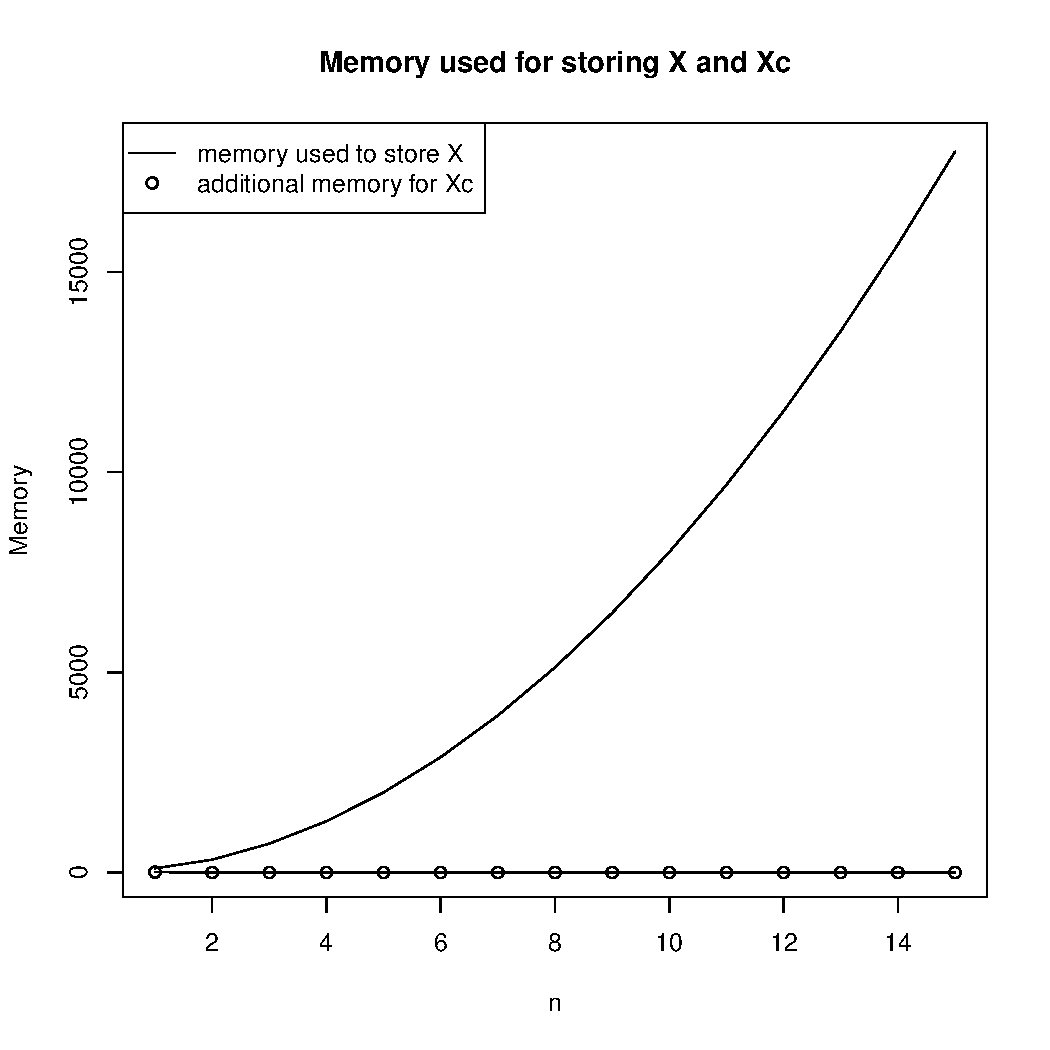
\includegraphics[width=\maxwidth]{figure/unnamed-chunk-2-1} 

\end{knitrout}
We can see that the additional memory used by the cholesky decomposition is not exactly zero, but 120 MB, which is much less than the memory used to store X. Apparently, the chol function uses more memory the first time it is computed in the loop.
\begin{knitrout}
\definecolor{shadecolor}{rgb}{0.969, 0.969, 0.969}\color{fgcolor}\begin{kframe}
\begin{alltt}
\hlstd{memX}
\end{alltt}
\begin{lstlisting}[basicstyle=\ttfamily,breaklines=true]
##  [1]   104248   320168   720168  1280168  2000168  2880168
##  [7]  3920168  5120168  6480168  8000168  9680168 11520168
## [13] 13520168 15680168 18000168
\end{lstlisting}
\begin{alltt}
\hlstd{memXc}
\end{alltt}
\begin{lstlisting}[basicstyle=\ttfamily,breaklines=true]
##  [1] 9376  120  120  120  120  120  120  120  120  120  120
## [12]  120  120  120  120
\end{lstlisting}
\end{kframe}
\end{knitrout}

%%%%%%%%%%%%%%%%%%%%%%%%%%%%%%%%%%%%%%%%%%%%%%%%%%%%%%%%%%%
\section{}
%%%%%%%%%%%%%%%%%%%%%%%%%%%%%%%%%%%%%%%%%%%%%%%%%%%%%%%%%%%

%%%%%%%%%%%%%%%%%%%
\subsection{}
%%%%%%%%%%%%%%%%%%%

\begin{knitrout}
\definecolor{shadecolor}{rgb}{0.969, 0.969, 0.969}\color{fgcolor}\begin{kframe}
\begin{alltt}
\hlcom{# Initialize Definite positive matrix}
\hlstd{n}\hlkwb{=}\hlnum{5000}
\hlstd{X0} \hlkwb{=} \hlkwd{matrix}\hlstd{(}\hlkwd{sample}\hlstd{(}\hlnum{0}\hlopt{:}\hlnum{9}\hlstd{,n}\hlopt{*}\hlstd{n,}\hlkwc{replace}\hlstd{=}\hlnum{TRUE}\hlstd{),n,n)}
\hlstd{X} \hlkwb{=} \hlkwd{crossprod}\hlstd{(X0,X0)}

\hlcom{# Initialize vector}
\hlstd{y} \hlkwb{=} \hlkwd{matrix}\hlstd{(}\hlkwd{sample}\hlstd{(}\hlnum{0}\hlopt{:}\hlnum{9}\hlstd{,n,}\hlkwc{replace}\hlstd{=}\hlnum{TRUE}\hlstd{),}\hlkwc{ncol}\hlstd{=}\hlnum{1}\hlstd{)}

\hlcom{# Compute elapsed time }
\hlcom{# Inverse and %*%}
\hlkwd{system.time}\hlstd{(\{Xi}\hlkwb{=}\hlkwd{solve}\hlstd{(X);xinverse}\hlkwb{=}\hlstd{Xi}\hlopt\hlstd{y\})}
\end{alltt}
\begin{lstlisting}[basicstyle=\ttfamily,breaklines=true]
##    user  system elapsed 
## 219.025   0.567 219.921
\end{lstlisting}
\begin{alltt}
\hlcom{# Solve}
\hlkwd{system.time}\hlstd{(\{xsolve}\hlkwb{=}\hlkwd{solve}\hlstd{(X,y)\})}
\end{alltt}
\begin{lstlisting}[basicstyle=\ttfamily,breaklines=true]
##    user  system elapsed 
##  25.208   0.088  25.322
\end{lstlisting}
\begin{alltt}
\hlcom{# Cholesky}
\hlkwd{system.time}\hlstd{(\{U}\hlkwb{=}\hlkwd{chol}\hlstd{(X);}
\hlstd{xchol}\hlkwb{=}\hlkwd{backsolve}\hlstd{(U,} \hlkwd{backsolve}\hlstd{(U, y,} \hlkwc{transpose} \hlstd{=} \hlnum{TRUE}\hlstd{))\})}
\end{alltt}
\begin{lstlisting}[basicstyle=\ttfamily,breaklines=true]
##    user  system elapsed 
##  17.192   0.073  17.280
\end{lstlisting}
\end{kframe}
\end{knitrout}

Here we have to look at the user time , which is the total time spent to compute the querries such as if everything were running in a single thread.
The naive way should be 6 times slower than the Cholesky. Here we see the time to solve the equations and not only the time spent to do the decomposition or the inverse matrix. The solve function calls the internal function $.Internal(La\_solve(a, b, tol))$.

%%%%%%%%%%%%%%%%%%%
\subsection{}
%%%%%%%%%%%%%%%%%%%
Are the results for b the same numerically for the different methods (up to machine precision)? 
\begin{knitrout}
\definecolor{shadecolor}{rgb}{0.969, 0.969, 0.969}\color{fgcolor}\begin{kframe}
\begin{alltt}
\hlcom{# Inverse and Solve}
\hlkwd{max}\hlstd{(xinverse}\hlopt{-}\hlstd{xsolve)}
\end{alltt}
\begin{lstlisting}[basicstyle=\ttfamily,breaklines=true]
## [1] 1.62359e-12
\end{lstlisting}
\begin{alltt}
\hlcom{# Cholesky and Solve}
\hlkwd{max}\hlstd{(xchol}\hlopt{-}\hlstd{xsolve)}
\end{alltt}
\begin{lstlisting}[basicstyle=\ttfamily,breaklines=true]
## [1] 1.6477e-05
\end{lstlisting}
\begin{alltt}
\hlcom{# Inverse and Cholesky}
\hlkwd{max}\hlstd{(xinverse}\hlopt{-}\hlstd{xchol)}
\end{alltt}
\begin{lstlisting}[basicstyle=\ttfamily,breaklines=true]
## [1] 1.771807e-05
\end{lstlisting}
\end{kframe}
\end{knitrout}


I relate this to the condition number of the calculation:
\begin{knitrout}
\definecolor{shadecolor}{rgb}{0.969, 0.969, 0.969}\color{fgcolor}\begin{kframe}
\begin{alltt}
\hlcom{# Inverse and Solve}
\hlstd{min_cond1}\hlkwb{=}\hlkwd{sqrt}\hlstd{(}\hlkwd{sum}\hlstd{((xinverse}\hlopt{-}\hlstd{xsolve)}\hlopt{^}\hlnum{2}\hlstd{))}\hlopt{/}\hlkwd{sqrt}\hlstd{(}\hlkwd{sum}\hlstd{((xsolve)}\hlopt{^}\hlnum{2}\hlstd{))}\hlopt{*}\hlnum{10}\hlopt{^}\hlnum{16}
\hlstd{min_cond1}
\end{alltt}
\begin{lstlisting}[basicstyle=\ttfamily,breaklines=true]
## [1] 49.81661
\end{lstlisting}
\begin{alltt}
\hlcom{# Cholesky and Solve}
\hlstd{min_cond2}\hlkwb{=}\hlkwd{sqrt}\hlstd{(}\hlkwd{sum}\hlstd{((xchol}\hlopt{-}\hlstd{xsolve)}\hlopt{^}\hlnum{2}\hlstd{))}\hlopt{/}\hlkwd{sqrt}\hlstd{(}\hlkwd{sum}\hlstd{((xinverse)}\hlopt{^}\hlnum{2}\hlstd{))}\hlopt{*}\hlnum{10}\hlopt{^}\hlnum{16}
\hlstd{min_cond2}
\end{alltt}
\begin{lstlisting}[basicstyle=\ttfamily,breaklines=true]
## [1] 1073477077
\end{lstlisting}
\begin{alltt}
\hlcom{# Inverse and Cholesky}
\hlstd{min_cond3}\hlkwb{=}\hlkwd{sqrt}\hlstd{(}\hlkwd{sum}\hlstd{((xinverse}\hlopt{-}\hlstd{xchol)}\hlopt{^}\hlnum{2}\hlstd{))}\hlopt{/}\hlkwd{sqrt}\hlstd{(}\hlkwd{sum}\hlstd{((xchol)}\hlopt{^}\hlnum{2}\hlstd{))}\hlopt{*}\hlnum{10}\hlopt{^}\hlnum{16}
\hlstd{min_cond3}
\end{alltt}
\begin{lstlisting}[basicstyle=\ttfamily,breaklines=true]
## [1] 1073477184
\end{lstlisting}
\end{kframe}
\end{knitrout}


%%%%%%%%%%%%%%%%%%%%%%%%%%%%%%%%%%%%%%%%%%%%%%%%%%%%%%%%%%%
\section{}
%%%%%%%%%%%%%%%%%%%%%%%%%%%%%%%%%%%%%%%%%%%%%%%%%%%%%%%%%%%

Since $\Sigma \in \mathbbm{M}_{p}(\mathbbm{R})$ is symmetric positive definite i.e. in $S^{++}_{p}(\mathbbm{R})$, ${\Sigma}^{-1}$ is also in $S^{++}_{p}(\mathbbm{R})$. Using Cholesky decomposition, we have:
\begin{equation}
\exists P \in \mathbbm{UT}^{+}_{p}(\mathbbm{R}) \hspace{.5cm}s.t.\hspace{.5cm} {\Sigma}= P^{T}P.
\end{equation}
Using the property that the inverse of an upper triangular matrix is an upper triangular matrix, we have:
\begin{equation}
{\Sigma}^{-1}= P^{-1}P^{-T}=U^{T}U \hspace{.5cm}with\hspace{.5cm} U=P^{-T} \in \mathbbm{UT}^{+}_{p}(\mathbbm{R}).
\end{equation}
Therefore, the generalized least squares problem becomes:
\begin{align}
&Find \hspace{.5cm} \hat{\beta} \hspace{.5cm} s.t. \hspace{.5cm} X^{T}U^{T}UX \hat{\beta}= X^{T}U^{T}UY.\nonumber\\
i.e. \hspace{.5cm} & Find \hspace{.5cm} \hat{\beta} \hspace{.5cm} s.t. \hspace{.5cm} (UX)^{T}(UX) \hat{\beta}= (UX)^{T}(UY).
\end{align}
Therefore, the generalized least squares model (GLS) is the ordinary least squares (OLS) with a change of basis characterized by $U$. In order to implement the GLS we first compute the Cholesky decomposition of $\Sigma$ in order to have P. Then, taking the inverse of the transpose of P, we get U which is used to change $X$ in $UX$ and $Y$ in $UY$. Finally, we use the Cholesky decomposition of $X$ in order to solve the OLS efficiently, like in the previous problem.\\ 
Even more efficiently, we can use the $backsolve$ function of R in order to get $UX$ and $UY$ directly from P.
\begin{knitrout}
\definecolor{shadecolor}{rgb}{0.969, 0.969, 0.969}\color{fgcolor}\begin{kframe}
\begin{alltt}
\hlstd{n}\hlkwb{=}\hlnum{100}
\hlstd{p}\hlkwb{=}\hlnum{10}
\hlstd{y}\hlkwb{=}\hlkwd{matrix}\hlstd{(}\hlkwd{runif}\hlstd{(n),}\hlkwc{nrow}\hlstd{=n,}\hlkwc{ncol}\hlstd{=}\hlnum{1}\hlstd{)}
\hlstd{X0}\hlkwb{=}\hlkwd{matrix}\hlstd{(}\hlkwd{runif}\hlstd{(n}\hlopt{*}\hlstd{n),n,n)}
\hlstd{S}\hlkwb{=}\hlstd{(X0}\hlopt{+}\hlkwd{t}\hlstd{(X0))}\hlopt{/}\hlstd{n}\hlopt{+}\hlkwd{diag}\hlstd{(n)}
\hlstd{X0}\hlkwb{=}\hlkwd{matrix}\hlstd{(}\hlkwd{runif}\hlstd{(n}\hlopt{*}\hlstd{n),n,n)}
\hlstd{X}\hlkwb{=}\hlstd{(X0}\hlopt{+}\hlkwd{t}\hlstd{(X0))}\hlopt{/}\hlstd{n}\hlopt{+}\hlkwd{diag}\hlstd{(n)}

\hlstd{gls} \hlkwb{=} \hlkwa{function}\hlstd{(}\hlkwc{X}\hlstd{,}\hlkwc{Y}\hlstd{,}\hlkwc{S}\hlstd{)\{}
  \hlcom{# X is a nxp matrix}
  \hlcom{# Y is a vector of length n}
  \hlcom{# S is a covariance matrix}
  \hlstd{P}\hlkwb{=}\hlkwd{chol}\hlstd{(S)}
  \hlstd{Xbis}\hlkwb{=}\hlkwd{backsolve}\hlstd{(P,X,}\hlkwc{transpose} \hlstd{=} \hlnum{TRUE}\hlstd{)}
  \hlstd{Ybis}\hlkwb{=}\hlkwd{backsolve}\hlstd{(P,Y,}\hlkwc{transpose} \hlstd{=} \hlnum{TRUE}\hlstd{)}
  \hlstd{V}\hlkwb{=}\hlkwd{chol}\hlstd{(}\hlkwd{tcrossprod}\hlstd{(Xbis,Xbis))}
  \hlkwd{backsolve}\hlstd{(Xbis,} \hlkwd{backsolve}\hlstd{(Xbis,} \hlkwd{crossprod}\hlstd{(Xbis,Ybis),} \hlkwc{transpose} \hlstd{=} \hlnum{TRUE}\hlstd{))}

\hlstd{\}}
\hlkwd{head}\hlstd{(}\hlkwd{gls}\hlstd{(X,y,S))}
\end{alltt}
\begin{lstlisting}[basicstyle=\ttfamily,breaklines=true]
##             [,1]
## [1,] -0.08432856
## [2,]  0.23824493
## [3,] -0.02879963
## [4,] -0.17175878
## [5,]  0.40518385
## [6,] -0.14102763
\end{lstlisting}
\end{kframe}
\end{knitrout}

%%%%%%%%%%%%%%%%%%%%%%%%%%%%%%%%%%%%%%%%%%%%%%%%%%%%%%%%%%%
\section{}
%%%%%%%%%%%%%%%%%%%%%%%%%%%%%%%%%%%%%%%%%%%%%%%%%%%%%%%%%%%
\subsection{}
Let $v \in \mathbbm{R^{p}} $ be a right singular vector of $X \in \mathbbm{M}_{n,p}(\mathbbm{R})$ and $\lambda \in \mathbbm{R}$ be the associated singular value.\\
$\exists u \in \mathbbm{R^{n}}$ such that:
\begin{equation}
Xv=\lambda u
\end{equation}
\begin{equation}
X^{T}u= \lambda v
\end{equation}
Then:
\begin{equation}
X^{T}Xv=X^{T}(\lambda u)=\lambda X^{T}u={\lambda}^{2}v
\end{equation}
Which proves that $v$ is an eigen vector of $X^{T}X$ associated with the eigenvalue $\lambda$ and associated eigenvalue is ${\lambda}^{2}$. There exists $p$ distinct singular values for $X$, so we have found $p$ distinct eigen values of $X^{T}X$. Therefore, reciprocally every eigenvalue of $X^{T}X$ can be expressed as the square of one right singular value of $X$.
\subsection{}
Let $X \in \mathbbm{M}_{n,p}(\mathbbm{R})$ and note $M$ the product $X^{T}X$. $M$ is clearly symmetric and belongs to $\mathbbm{M}_{p}(\mathbbm{R})$. Therefore let's note $(v_{i})_{1\leq i\leq p}$ its eigen vectors respectively associated with the eigenvalues $({\sigma}_{i})_{1\leq i\leq p}$. From before we have the existence of 
$({\lambda}_{i})_{1\leq i\leq p}$ such that $\forall i,{\lambda}_{i}^{2} = {\sigma}_{i} $.
\begin{equation}
\forall x \in \mathbbm{R^{p}, \exists ({\sigma}_{i})_{1\leq i\leq p} } \hspace{.5cm}\mbox{ such that }\hspace{.5cm} x=\sum_{i=0}^{p}{\alpha}_{i}v_{i}
\end{equation}
Then using the orthogonality of the eigen vectors of M we have $\forall x \in \mathbbm{R^{p}}$:
\begin{align}
x^{T}Mx&=(\sum_{i=0}^{p}{\alpha}_{i}v_{i})^{T}M(\sum_{i=0}^{p}{\alpha}_{i}v_{i}) \nonumber\\
&=(\sum_{i=0}^{p}{\alpha}_{i}v_{i})^{T}(\sum_{i=0}^{p}{\alpha}_{i}{\lambda}_{i}^{2}v_{i})
\nonumber\\
&=\sum_{i=0}^{p}{\alpha}_{i}^{2}{\lambda}_{i}^{2}{||v_{i}||}^{2} \geq 0
\end{align}
Therefore M is a symmetric positive matrix.
\subsection{}
Equivalently:
\begin{align}
Xv=\lambda v  &\iff Zv=\lambda v+ cv \nonumber\\
&\iff Zv=(\lambda + c)v
\end{align}
Therefore the eigenvalues of $Z$ are $\{{\lambda+c | \lambda \in \mathbbm{ S}_{p}(\mathbbm{R})}\}$. In order to compute these eigenvalues we can add $c$ to every eigenvalue of $X$. The complexity here is exactly $n$ additions.




\end{document}





